\subsection{Radio Frequency Module Difference Test} % (fold)
\label{cha:radio_frequency_module_difference_test}
In tests using the \gls{rf}-modules the difference in build quality and performance between the modules is a significant factor, and could be a source of error.
A test must be performed which investigates these differences, so that the other test results can be validated.

\subsubsection*{Test setup}
To test all \gls{rf}-modules available to the group two Arduinos are used; one as the receiver where they are configured as seen on \myref{fig:Receiver} and the other as the transmitter as seen on \myref{fig:Transmitter}.
The \gls{rf}-modules are then switched in and out of breadboards connected to said Arduinos so that both receiver and transmitter modules can be tested.
Furthermore, a third Arduino is used to verify the results of each module.
The software on the Arduinos is the same as in the test in \myref[name]{cha:radio_frequency_module_reception_test}, i.e. a transmitting part which sends 100 unique packages and a receiving part which register any package loss. 
Modules are tested to find a transmitter that shows little to no package loss, thereafter every receiver is tested using the \enquote*{good} transmitter; with good meaning a package loss close to 0 \%, at most 2 \%.
The same thing is done to test the transmitters, i.e. a good receiver is used.

\begin{figure}[h]
\centering
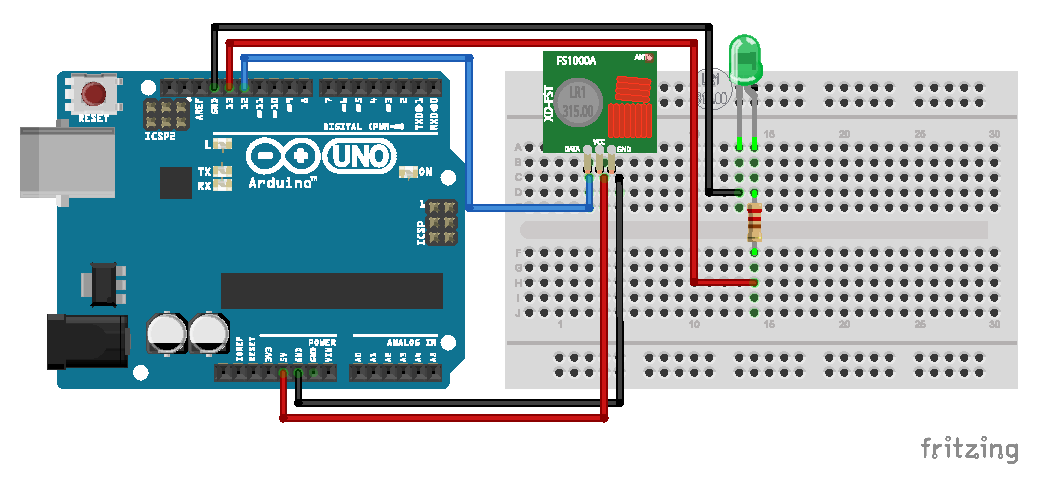
\includegraphics[width=\linewidth]{Figures/Fritzing/Transmitter.pdf} 
\caption{Graphical circuit diagram of an Arduino with a transmitter.}
\label{fig:Transmitter}   
\end{figure}

\begin{figure}[h]
\centering
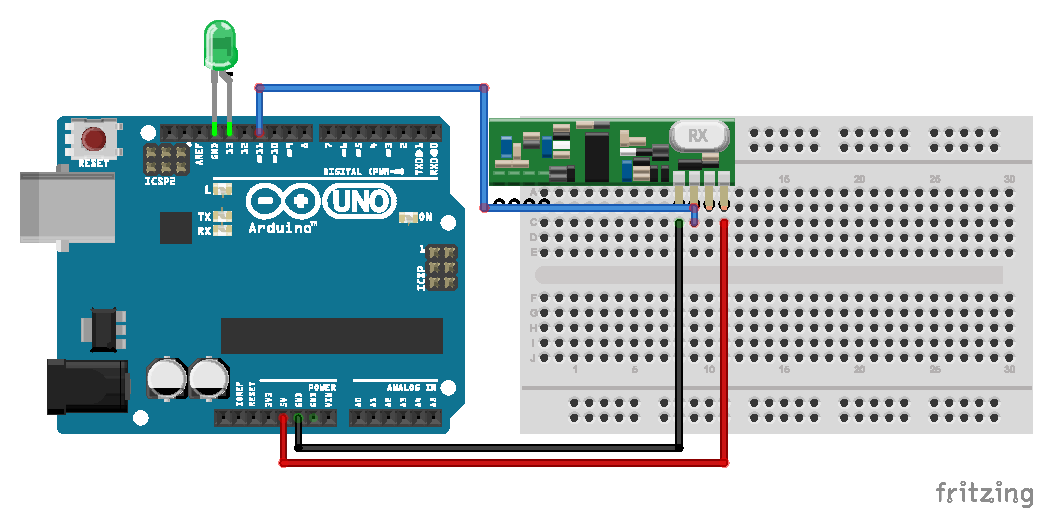
\includegraphics[width=\linewidth]{Figures/Fritzing/Receiver.pdf} 
\caption{Graphical circuit diagram of an Arduino with a receiver.}
\label{fig:Receiver}   
\end{figure}

This approach is then repeated with different good receivers and transmitters, to ensure a more fair test environment, with different combinations of modules.
The results have been plotted in one bar chart, with the results of the different transmitters in the leftmost half, and the results of the different receivers in the rightmost half.

\begin{figure}[H]
\centering
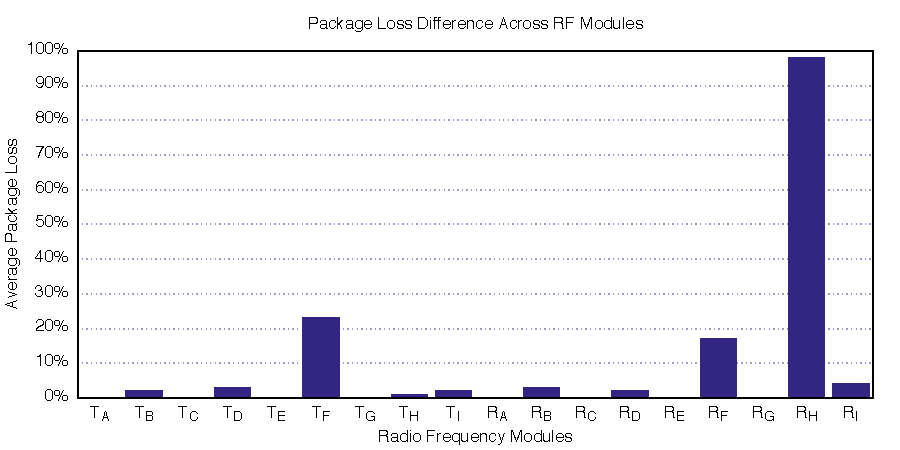
\includegraphics[width=\linewidth]{Figures/Graphs/diff_graph.pdf}
\centering
\caption{The average package loss inflicted by the radio frequency modules.\\ \textsf{T}\textsubscript{\textit{device}} denotes transmitters and \textsf{R}\textsubscript{\textit{device}} denotes receivers.}    
\label{fig:trans_diff}       
\end{figure} 

\subsubsection*{Conclusion}
When looking at the results of this test, it is clear that some of the modules were worse at transmitting or receiving data.
Transmitter \textsf{T\textsubscript{F}} inflicted an average package loss over 20 \%, and receiver \textsf{R\textsubscript{H}} failed to receive more than 98 \% of the packages on average.
Moreover, receiver \textsf{R\textsubscript{F}} had an average package loss just below 20 \%.
To ensure the validity of other tests using the RF Modules, the group will exclude the three faulty modules (transmitter \textsf{T\textsubscript{F}}, receiver \textsf{R\textsubscript{H}}, and receiver \textsf{R\textsubscript{F}}) from these tests.
% chapter radio_frequency_module_difference_test (end) 
